\everymath{\displaystyle}
\documentclass{beamer}
% \documentclass[handout]{beamer}

%\usepackage[pdftex]{color,graphicx}
\usepackage{amsmath,amssymb,amsfonts}

\mode<presentation>
{
  % \usetheme{Darmstadt}
  % \usetheme[hideothersubsections]{Hannover}
  % \usetheme[hideothersubsections]{Goettingen}
  \usetheme[hideothersubsections, right]{Berkeley}

  \usecolortheme{seahorse}
  % \usecolortheme{dolphin}
  \usecolortheme{rose}
  % \usecolortheme{orchid}

  \useinnertheme[shadow]{rounded}

  % \setbeamercovered{transparent}
  \setbeamercovered{invisible}
  % or whatever (possibly just delete it)
}

\mode<handout>{
  \setbeamercolor{background canvas}{bg=black!5}
  \usepackage{pgfpages}
  \pgfpagesuselayout{4 on 1}[a4paper,border shrink=5mm, landscape]
}

\usepackage[brazilian]{babel}
% or whatever

% \usepackage[latin1]{inputenc}
\usepackage[utf8]{inputenc}
% or whatever

\usepackage{times}
%\usepackage[T1]{fontenc}
% Or whatever. Note that the encoding and the font should match. If T1
% does not look nice, try deleting the line with the fontenc.


\title[Significância] % (optional, use only with long paper titles)
{Significância Estatística}

\subtitle
{O p-valor e Testes de Hipóteses} % (optional)

\author%[] % (optional, use only with lots of authors)
{Felipe Figueiredo}% \and S.~Another\inst{2}}
% - Use the \inst{?} command only if the authors have different
%   affiliation.

\institute[] % (optional, but mostly needed)
{
}
  % \inst{1}%
  % Department of Computer Science\\
  % University of Somewhere
  % \and
  % \inst{2}%
  % Department of Theoretical Philosophy\\
  % University of Elsewhere}
% - Use the \inst command only if there are several affiliations.
% - Keep it simple, no one is interested in your street address.

\date%[] % (optional)
{}

% \subject{Talks}
% This is only inserted into the PDF information catalog. Can be left
% out. 



% If you have a file called "university-logo-filename.xxx", where xxx
% is a graphic format that can be processed by latex or pdflatex,
% resp., then you can add a logo as follows:

\pgfdeclareimage[height=1.6cm]{university-logo}{../logo}
\logo{\pgfuseimage{university-logo}}



% Delete this, if you do not want the table of contents to pop up at
% the beginning of each subsection:
\AtBeginSubsection[]
%\AtBeginSection[]
{
  \begin{frame}<beamer>{Sumário}
    \tableofcontents[currentsection,currentsubsection]
  \end{frame}
}


% If you wish to uncover everything in a step-wise fashion, uncomment
% the following command: 

% \beamerdefaultoverlayspecification{<+->}


\begin{document}

\begin{frame}
  \titlepage
\end{frame}

\begin{frame}{Sumário}
  \tableofcontents
  % You might wish to add the option [pausesections]
\end{frame}


%% Template
% \section{}

% \subsection{}

% \begin{frame}{}
%   \begin{itemize}
%   \item 
%   \end{itemize}
% \end{frame}

% \begin{frame}
%   \begin{columns}
%     \begin{column}{5cm}
%     \end{column}
%     \begin{column}{5cm}
%     \end{column}
%   \end{columns}
% \end{frame}

% \begin{frame}{}
%   \includegraphics[height=0.4\textheight]{file1}
%   \includegraphics[height=0.4\textheight]{file2}
%   \includegraphics[height=0.4\textheight]{file3}
%   \begin{figure}
%     \caption{}
%   \end{figure}
% \end{frame}

% \begin{frame}{}
%   \begin{definition}
%   \end{definition}
%   \begin{example}
%   \end{example}
%   \begin{block}{Exercício}
%   \end{block}
% \end{frame}

% \section{O p-valor}

\section{Testes de Hipóteses}

\subsection{Hipóteses}

\begin{frame}{Introdução}
  \begin{block}{Dante Alighieri}
    \small
    {\em ``A meio do caminho, ou seja, da duração expectável de sua vida, Dante, consciente de se haver desviado do reto procedimento, encontra-se perdido numa alegórica 'Selva Perdida'.

      \bigskip
    Encontra aí a figura de Virgílio, o poeta latino que (...) vem se lhe oferecer como guia para o Inferno e o Purgatório onde, pelo exemplo dos pecadores e de suas penas, Dante poderá encontrar o caminho da sua salvação.''}
  \end{block}
\end{frame}

\begin{frame}{Hipóteses científicas}
  \begin{itemize}
  \item Podemos tomar decisões baseado nos dados de um experimento
    (amostra).
  \item Para isto, precisamos de um critério sistemático e rigoroso
    que possa aferir o quanto os dados suportam esta decisão.
  \item Usando os conceitos de probabilidades, poderemos ainda
    calcular a probabilidade de que esta decisão esteja errada.
  \end{itemize}
  \begin{block}{}
    {\bf Hipóteses devem ser falseáveis, portanto formuladas como afirmações}.
  \end{block}
\end{frame}

\begin{frame}[label=exemplo1]{Exemplo 1}
  \begin{exampleblock}{Exemplo}
    Um neurologista está testando o efeito de uma droga no tempo de
    resposta de um certo estímulo neurológico. Para isto, ele injeta
    uma dose da droga em \alert{100} ratos, cria os estímulos
    neurológicos e observa o tempo de resposta em cada animal. O
    neurologista sabe que o tempo de resposta médio de ratos que não
    receberam a droga é de \alert{1.2 segundos}. O tempo de resposta
    médio dos ratos injetados foi de \alert{1.05 segundos}, com desvio
    padrão amostral de \alert{0.5 segundos}. Você acha que a droga tem
    efeito no tempo de resposta do estímulo?
  \end{exampleblock}
Fonte: Khan Academy
\end{frame}

\begin{frame}{Pergunta}
  \begin{block}{Pense...}
    Como você formularia a hipótese do exemplo anterior?

    \bigskip
    Que possíveis conclusões você pode chegar com esse experimento?
  \end{block}

  Vamos resolvê-lo mais à frente.
\end{frame}

\begin{frame}{Hipóteses estatísticas}
  \begin{definition}
    Em Estatística, uma \alert{hipótese} é uma afirmação sobre uma
    característica de uma população, tipicamente o valor de um
    parâmetro.
  \end{definition}
  \begin{definition}
    Um \alert{teste de hipótese} (ou teste de significância) é um
    procedimento sistemático para testar uma afirmação sobre uma
    característica de uma população.
  \end{definition}
\end{frame}

\begin{frame}{Identificando hipóteses}
  \begin{itemize}
  \item Uma hipótese estatística deve ser testável frente a dados
    obtidos de um experimento.
  \end{itemize}
  \begin{exampleblock}{Exemplo}
    Um jornalista alega que a maior parte dos motoristas atravessa o
    sinal vermelho.
  \end{exampleblock}
  \begin{exampleblock}{Exemplo}
    Pesquisadores afirmam que a temperatura corporal média de adultos
    sadios não ultrapassa 37$^o$C.
  \end{exampleblock}
\end{frame}

\begin{frame}{Identificando hipóteses}
  \begin{itemize}
  \item Para efetuar um teste de hipóteses é necessária a formulação  de uma \alert{hipótese nula} e uma \alert{hipótese alternativa}.
  \item A hipótese nula ($H_0$) é a hipótese que não há efeito real.
  \item A hipótese alternativa ($H_1$ ou $H_a$) é a hipótese de interesse científico (há efeito).
  \end{itemize}
\end{frame}

\begin{frame}{Identificando hipóteses}
  \begin{block}{Atenção}
    A lógica do teste de hipóteses é o \alert{inverso} do que se esperaria, ou seja, ao invés de testar a hipótese de interesse, vamos {\em testar a hipótese nula} -- e tentar rejeitá-la.

\bigskip
{\bf Mantenha isso em mente daqui a para a frente.}
  \end{block}
\end{frame}

\begin{frame}{Identificando hipóteses}
  \begin{block}{Roteiro}
    \begin{enumerate}
    \item Identificar a afirmação a ser testada e expressá-la em forma simbólica
    \item Expressar em forma simbólica a afirmação que deve ser
      verdadeira, caso a afirmação de interesse seja falsa
    % \item Das duas expressões obtidas, a hipótese $H_0$ será a que
    %   contém igualdade $=$, enquanto a $H_1$ será a que contém um
    %   sinal de $<$, $>$ ou $\ne$.
    \end{enumerate}
  \end{block}
\end{frame}

\begin{frame}{Identificando hipóteses}
  \begin{exampleblock}{Exemplo}
    Formulação verbal:\\
    A proporção de motoristas que admitem atravessar o sinal vermelho
    é maior que 50\%.\\
    \bigskip
    Formulação matemática:\\
    \begin{displaymath}
      H_0: p=0.5
    \end{displaymath}
    \begin{displaymath}
      H_1: p>0.5
    \end{displaymath}
  \end{exampleblock}
\end{frame}

\begin{frame}{Identificando hipóteses}
  \begin{exampleblock}{Exemplo}
    Formulação verbal:\\
    A altura média de jogadores profissionais de basquete é de no
    máximo 2.20m.\\
    \bigskip
    Formulação matemática:\\
    \begin{displaymath}
      H_0: \mu = 2.20
    \end{displaymath}
    \begin{displaymath}
      H_1: \mu < 2.20
    \end{displaymath}
  \end{exampleblock}
\end{frame}

\begin{frame}{Identificando hipóteses}
  \begin{exampleblock}{Exemplo}
    Formulação verbal:\\
    A dose média contida em um comprimido de paracetamol é de 750mg.\\
    \bigskip
    Formulação matemática:\\
    \begin{displaymath}
      H_0: \mu = 750
    \end{displaymath}
    \begin{displaymath}
      H_1: \mu \ne 750
    \end{displaymath}
  \end{exampleblock}
  \begin{center}
      \only<2->{
\includegraphics[height=2cm]{Jackie-Chan-WTF}}
  \end{center}
\end{frame}

\begin{frame}{Identificando a região crítica}
  Em geral...
  \begin{itemize}
  % \item Para identificar a região crítica (ou região de rejeição) do
  %   teste, devemos observar se o teste é unicaudal (à esquerda ou à
  %   direita) ou bicaudal.
  \item Se $H_1$ é do tipo $\ne$, o teste é bicaudal (ou bilateral).
  \item Se $H_1$ é do tipo $<$, o teste é unicaudal (ou unilateral) à esquerda.
  \item Se $H_1$ é do tipo $>$, o teste é unicaudal à direita.
  \end{itemize}
\end{frame}

\subsection{Significância}
\begin{frame}{Significância}
  \begin{itemize}
  \item A {\bf significância} do estudo deve ser arbitrada antes do experimento (planejamento)
  \item Está associada aos erros induzidos pela variabilidade experimental
  \item Ou seja, mesmo fazendo tudo certo, você pode ser induzido a chegar numa conclusão errada ao acaso!
  \item Isso pode ocorrer de duas maneiras diferentes...
  \end{itemize}
\end{frame}

\begin{frame}{Tipos de erros em testes de hipóteses}
  \begin{definition}
    Um \alert{erro do tipo I} ocorre se a hipótese nula for rejeitada
    quando é verdadeira.
  \end{definition}
  \begin{definition}
    Um \alert{erro do tipo II} ocorre se a hipótese não for rejeitada
    quando for falsa.
  \end{definition}
\end{frame}

\begin{frame}{Observe}
  \begin{block}{A questão importante aqui é:}
    MESMO SE a hipótese nula {\bf for verdadeira}, ainda assim você pode observar (ao acaso) uma diferença como resultado do experimento.

    \bigskip
    (ex., muita variabilidade, amostras pequenas, etc.).

    \bigskip
    {\bf Isso} é o erro tipo I. Trabalhamos para que isso seja raro (não mais que 5\% das vezes).
  \end{block}
\end{frame}

\begin{frame}{Tipos de erros em testes de hipóteses}
  \begin{block}{}
    \begin{tabular}{c||c|c}
      Decisão / Verdade & $H_0$ é verdadeira & $H_0$ é falsa \\
      \hline
      \hline
      Não rejeitar $H_0$ & Decisão correta & Erro do tipo II\\
      \hline
      Rejeitar $H_0$ & Erro do tipo I & Decisão correta\\
    \end{tabular}
  \end{block}
  \begin{itemize}
  \item Erro do tipo I = falso positivo
  \item Erro do tipo II = falso negativo
  \end{itemize}
\end{frame}

\begin{frame}{Nível de significância}
  \begin{definition}
    O \alert{nível de significância} de um teste de hipótese é sua
    probabilidade máxima admissível para cometer um erro do tipo
    I. Ele é denotado por $\alpha$.

    \bigskip
    Está associado com o nível de confiança.
  \end{definition}
  \begin{definition}
    A probabilidade de se cometer um erro do tipo II é denotada por
    $\beta$.

    \bigskip Está associado com o poder estatístico do teste (futuro).
  \end{definition}
  % \begin{itemize}
  % % \item O valor $1-\beta$ é chamado o \alert{poder do teste}.
  % % \item Devemos controlar o erro do tipo I, isto é, 
  % % \item Quando você decresce $\alpha$, você provavelmente aumentará $\beta$.
  % \end{itemize}
\end{frame}

\begin{frame}{Componentes de um teste de hipóteses}
  São necessários para um teste de hipóteses:
  \begin{itemize}
  \item As hipóteses nula e alternativa
  \item O nível de significância
  \item A região crítica (tipo de teste)
  \item A estatística de teste (softwares especializados)
%  \item 
  \end{itemize}
  \begin{block}{Observação}
    O teste unicaudal {\bf divide} a probabilidade de erro à esquerda (valores menores) e à direita (valores maiores).

    \bigskip
    Assim, 5\% de significância num teste unicaudal corresponde à 2.5\% (metade) da significância bicaudal.

    \bigskip
    Mais detalhes no cap 10.
  \end{block}
\end{frame}

\begin{frame}{Rejeitar hipóteses}
  \begin{block}{Importante}
    Observe que o teste de hipótese nunca deve \alert{aceitar} uma
    hipótese nula, apenas rejeitá-la ou deixar de rejeitá-la.
  \end{block}
\end{frame}

\subsection{O p-valor}

\begin{frame}{O p-valor}
  \begin{definition}
    Assumindo que a hipótese nula seja verdadeira, o \alert{p-valor}
    de um teste de hipóteses é a probabilidade de se obter uma
    estatística amostral com valores tão extremos, ou mais extremos
    que aquele observado.
  \end{definition}

O p-valor \alert{é}:
  \begin{itemize}
  \item Uma estatística (i.e., depende da amostra - dados e tamanho)
  \item A probabilidade (condicional) de se observar o resultado ao
    acaso \alert{dado que} a $H_0$ é verdadeira.
  \item Uma medida da força da evidência contra a $H_0$.
  \end{itemize}
\end{frame}

\begin{frame}{O p-valor}
  \begin{block}{Como utilizar}
    \begin{itemize}
    \item Quanto menor o p-valor, mais evidências para rejeitar a
      hipótese nula.
    \item O ponto de corte mais utilizado é a significância de 5\%
    \item Assim, qualquer $p \le 0.05$ é estatisticamente significante.
    \end{itemize}
  \end{block}
\end{frame}

% \begin{frame}{O p-valor}
%   \begin{figure}
%     \centering
%       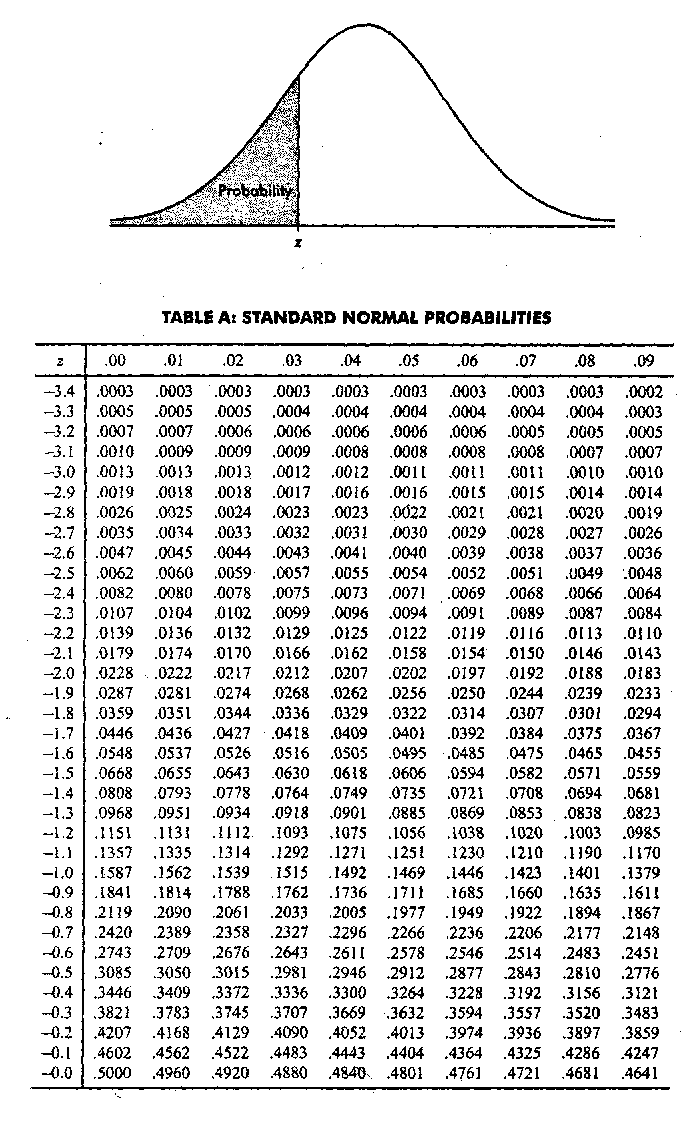
\includegraphics[height=0.9\textheight]{TH_II/z_table}
%   \end{figure}
% \end{frame}

\againframe{exemplo1}

\begin{frame}{Exemplo}
  \begin{block}{Pense...}
    \begin{itemize}
    \item A hipótese científica é que a droga diminui o tempo de resposta.
    \item Como você formularia a hipótese estatística ($H_1$)?
      \begin{enumerate}
      \item $H_0: \mu = 1.2, H_1: \mu \ge 1.2$ (teste unicaudal à direita)
      \item $H_0: \mu = 1.2, H_1: \mu < 1.2$ (teste unicaudal à esquerda)
      \item $H_0: \mu = 1.2, H_1: \mu \ne 1.2$ (teste bicaudal)
      \item $H_0: \mu \ge 1.2, H_1: \mu = 1.2$ (teste unicaudal à esquerda)
      \end{enumerate}

      Resposta: \only<2->{\bf Opção 2}
%    \item Qual seria a hipótese nula ($H_0$) a ser rejeitada, caso a droga seja eficaz?
    \end{itemize}
  \end{block}
\end{frame}

\begin{frame}{Exemplo 1}
  \begin{exampleblock}{Exemplo}
    \begin{itemize}
    \item Dados: $\mu = 1.2, \bar{x} = 1.05, s = 0.5, n=100$
    \item $H_0: \mu = 1.2, H_1: \mu < 1.2$ (teste unicaudal à esquerda)
    % \item $n$ é grande ($n > 30$), então usamos $\sigma \approx s$ , e
    %   fazemos o teste Z:
    % \item $Z = \frac{1.05 - 1.2}{\frac{0.5}{\sqrt{100}}} = -3$
    \item O teste Z aplicado a este problema retorna $p=0.0013$
    \item<2-> Como $p < 0.05$, concluímos que há evidência para rejeitar
      $H_0$.
    \item<2-> {\bf Resultado: O tempo de resposta médio é \alert{significativamente} menor.}
    \item<2-> {\bf Conclusão: \only<3->{há evidências que a droga diminui o tempo de resposta (...)}}
    \end{itemize}
  \end{exampleblock}
\end{frame}

\begin{frame}{O p-valor}
  Cuidado! O p-valor \alert{não é}:
  \begin{itemize}
  \item a probabilidade de que a hipótese nula seja verdadeira
  \item a probabilidade de que a diferença observada seja devido ao
    acaso
  \end{itemize}
  \begin{block}{}
    Estes são erros comuns de interpretação.

    O p-valor assume que (1) a hipótese é verdadeira, e (2) que a
    única causa da diferença é devida ao acaso, portanto não pode ser
    usado para concluir suas próprias premissas.
  \end{block}
  \begin{block}{}
    ``The concept of a p value is not simple and any statements
    associated with it must be considered cautiously.''

    Dorey, F. 2010 Clin Orthop Relat Res.
  \end{block}
\end{frame}

\section{Encerramento}

\begin{frame}{Leitura pós-aula e exercícios selecionados}
  \small
  \begin{block}{Leitura obrigatória}
%    \small
    \begin{itemize}
    \item Capítulo 10.
    \item Capítulo 11.
    \end{itemize}
  \end{block}
  \begin{block}{Exercícios selecionados}
%    \small
  \begin{itemize}
  \item Cap 10: todos.
  \item Cap 11: todos.
  \end{itemize}

\end{block}
\begin{block}{Leitura recomendada (links na página da disciplina)}
\tiny
  \begin{itemize}
  \item Motulsky, (2014) chap 19, Interpreting a Result That Is Not Statistically Significant
  \item Dorey, F (2010) In Brief: The P Value: What Is It and What Does It Tell You?
  \item Gardner, MJ; Altman, DG (1986) Confidence intervals rather than P values: estimation rather than hypothesis testing.
  \end{itemize}
\end{block}
\end{frame}

\end{document}
